\documentclass[12pt]{article}
%\usepackage[T1]{fontenc}
\usepackage{cite}
\usepackage[letterpaper,left=1in,right=1in,top=1in,bottom=1in]{geometry}
\setlength{\parindent}{15pt} % Default is 15pt.
\usepackage{setspace}
\usepackage{courier}
\usepackage{enumitem}
\usepackage{amsmath}
\usepackage{graphicx}
\usepackage{placeins}
%\onehalfspacing
\usepackage{color}

\pretolerance=10000
\tolerance=2000 
\emergencystretch=10pt

\usepackage{listings}
\definecolor{mygreen}{rgb}{0,0.6,0}
\definecolor{mygray}{rgb}{0.5,0.5,0.5}
\definecolor{mymauve}{rgb}{0.58,0,0.82}

\lstset{ %
	backgroundcolor=\color{white},   % choose the background color; you must add \usepackage{color} or \usepackage{xcolor}
	basicstyle=\scriptsize,        % the size of the fonts that are used for the code
	breakatwhitespace=false,         % sets if automatic breaks should only happen at whitespace
	breaklines=true,                 % sets automatic line breaking
	captionpos=b,                    % sets the caption-position to bottom
	commentstyle=\color{mygreen},    % comment style
	deletekeywords={...},            % if you want to delete keywords from the given language
	escapeinside={\%*}{*)},          % if you want to add LaTeX within your code
	extendedchars=true,              % lets you use non-ASCII characters; for 8-bits encodings only, does not work with UTF-8
	frame=single,                    % adds a frame around the code
	keepspaces=true,                 % keeps spaces in text, useful for keeping indentation of code (possibly needs columns=flexible)
	keywordstyle=\color{blue},       % keyword style
	language=Octave,                 % the language of the code
	morekeywords={*,...},            % if you want to add more keywords to the set
	numbers=left,                    % where to put the line-numbers; possible values are (none, left, right)
	numbersep=5pt,                   % how far the line-numbers are from the code
	numberstyle=\tiny\color{mygray}, % the style that is used for the line-numbers
	rulecolor=\color{black},         % if not set, the frame-color may be changed on line-breaks within not-black text (e.g. comments (green here))
	showspaces=false,                % show spaces everywhere adding particular underscores; it overrides 'showstringspaces'
	showstringspaces=false,          % underline spaces within strings only
	showtabs=false,                  % show tabs within strings adding particular underscores
	stepnumber=2,                    % the step between two line-numbers. If it's 1, each line will be numbered
	stringstyle=\color{mymauve},     % string literal style
	tabsize=2,                       % sets default tabsize to 2 spaces
}

\begin{document}
	
	\title{CS 5220: Homework 2}
	\date{\today}
	\author{Group 19: Robert Carson (rac428), Robert Chiodi (rmc298), Sam Tung (sat83)}
	\maketitle
		
	\section{Initial Profiling}
	In order to perform initial profiling of the code before any improvements are made, Intel's VTUNE was used via the terminal command line on Totient. In an attempt to get the most accurate results (taken with a large sample size), we decided to gather data while running the large wave simulation, invoked with the command \texttt{make big}. Information collected from VTUNE's 'advanced-hotspots' option is used in our analysis.
		\subsection{Whole Program - Advanced Hotspots}
		First, hotspots in the entire program were examined in order to determine where our efforts should be directed. The time taken in the top 10 most time consuming functions can be seen below in Figure~\ref{top10}. Of these, it is clear that most of our optimization efforts should be directed to the functions \texttt{limited\_derivs}, \texttt{compute\_step}, and \texttt{compute\_fg\_speeds}. These functions were then examined individually, once again using VTUNE on our advanced-hotspots collection.
		\begin{figure}[h]
			\begin{center}
				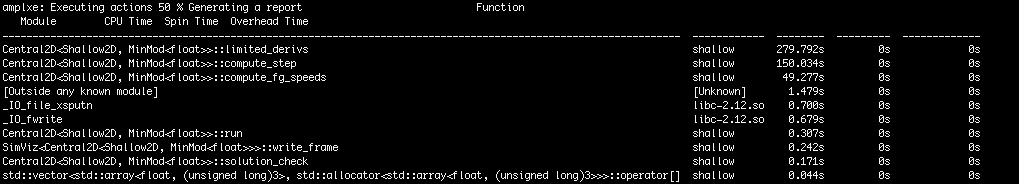
\includegraphics[width=0.7\columnwidth]{top10}
				\caption{Top 10 most time consuming functions in the wave simulation. Generated using Intel's VTUNE on Totient.}
				\label{top10}
			\end{center}
		\end{figure}
		\subsection{\texttt{limited\_derivs} - Advanced Hotspots}
		The function \texttt{limited\_deriv} is used to calculate the fluxes into and out of each cell in order to advance to the next time step. This involves a three point computational stencil in each direction and loops through the entire domain interior (the whole domain except for those where boundary conditions are applied). Each point requires $\mathtt{du.size()}\times 9$ floating point operations as well as $\mathtt{du.size()} \times 2$ calls to the intrinsic function $\mathtt{min}$. Sadly, the hotspot analysis on the \texttt{limited\_deriv} function, shown in Figure~\ref{init_lim_deriv}, does not give any hints on possible optimizations or bottle necks.
		
		\begin{figure}[h]
			\begin{center}
				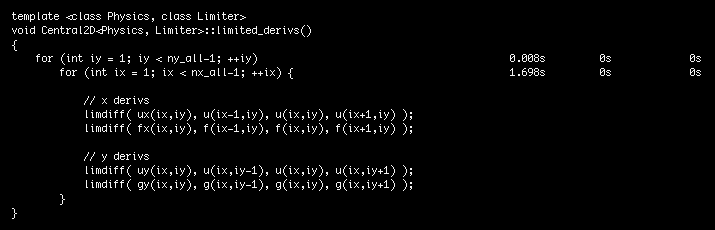
\includegraphics[width=0.7\columnwidth]{init_lim_deriv}
				\caption{Time taken to perform each loop present in \texttt{limited\_derivs}.}
				\label{init_lim_deriv}
			\end{center}
		\end{figure}
		
		\subsection{\texttt{compute\_step} - Advanced Hotspots}
		The purpose of \texttt{compute\_step} is to update the wave equation to the next time step using a predictor-corrector method. First, the fluxes are calculated in the prediction. Next, the corrector step uses the predicted fluxes, the differences in velocities, and the current velocities to advance to the next time state. Luckily, VTUNE's report is more helpful than in the previous case, and provides extensive timings for this function, shown in Figure~\ref{init_compute_step}. The calculation in the corrector step can be seen to be the most expensive cost of the function. It is important to note, however, that the predictor step and copying of the solution to the \texttt{u} array sum to half of the function's cost.
		\begin{figure}[h]
			\begin{center}
				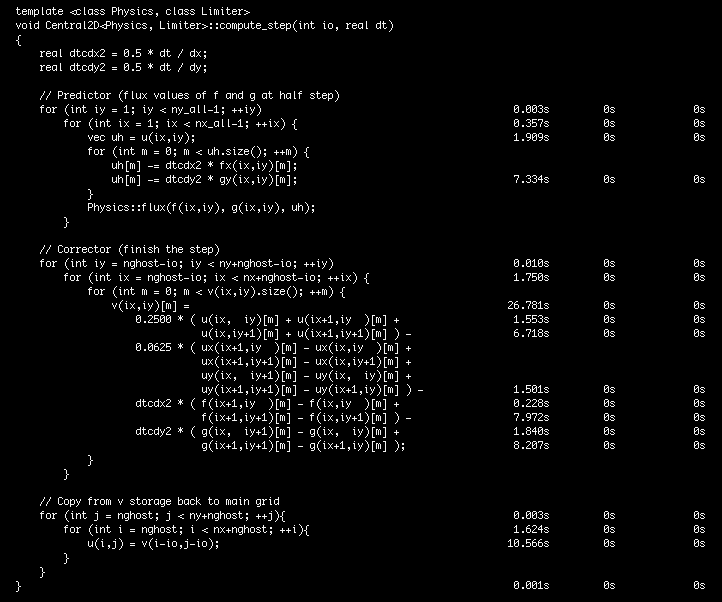
\includegraphics[width=0.7\columnwidth]{init_compute_step}
				\caption{Time taken to perform each loop present in \texttt{compute\_step}.}
				\label{init_compute_step}
			\end{center}
		\end{figure}	
		
		\subsection{\texttt{compute\_fg\_speeds} - Advanced Hotspots}
		The function of \texttt{compute\_fg\_speeds} has two primary responsibilities: to update the cell centered fluxes, \texttt{f} and \texttt{g}, and to calculate the maximum speed in the domain, allowing dynamic adjustment of the time step in order to satisfy the CFL condition and ensure numerical stability. The timing data for this function can be seen in Figure~\ref{init_compute_fg_speeds}. While the most time consuming portion of the code is most likely the calculation of the fluxes and wave speed (both of which are in the \texttt{Shallow2d} structure), the calls to the intrinsic function \texttt{max} also represent a non-trivial amount of time. 	
		\begin{figure}[h]
			\begin{center}
				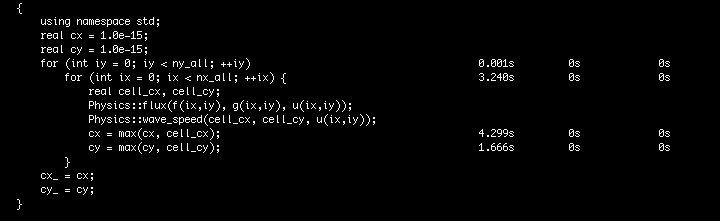
\includegraphics[width=0.7\columnwidth]{init_compute_fg_speeds}
				\caption{Time taken to perform each loop present in \texttt{compute\_fg\_speeds}.}
				\label{init_compute_fg_speeds}
			\end{center}
		\end{figure}	
		
	\section{Parallelization}
	While we are aware that the optimal programming of this code will not wholly be due to parallelization by OpenMP, it is most certainly necessary. Furthermore, future tuning and optimization of the code may change depending on whether the code is run serially or parallel. For these reason, we first decided to parallelize the code and compare it's performance against the initial, serial code.
		\subsection{Naive Implementation of OpenMP}
		First, a naive implementation of OpenMP using pragmas was used. This involved placing \texttt{#pragma omp parallel for} in front of the start of each for loop in the functions \texttt{init}, \texttt{apply\_periodic}, \texttt{compute\_fg\_speeds}, \texttt{limited\_derivs}, and \texttt{compute\_step}. This proved to improve performance significantly when run on one node of Totient (24 threads), as seen in Figure~\ref{naive_omp}. 
		
		! Will include rest of part on how it performed better. Need to run 'big' simulation.
		
		\begin{figure}[h]
			\begin{center}
				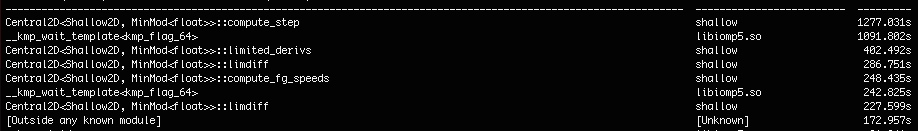
\includegraphics[width=0.7\columnwidth]{naive_omp}
				\caption{Timing of entire simulation using naive implementation of OpenMP parallelized for-loops. Generated using Intel's VTUNE on Totient.}
				\label{naive_omp}
			\end{center}
		\end{figure}
		
		\subsection{OpenMP for with \texttt{collapse}}
		OpenMP parallel for also has the \texttt{collapse} option, which essentially informs OpenMP how many nested loops are present. By knowing this, OpenMP is able to section both loops to run on multiple processors, creating blocks for each processor to work on. Results when using \texttt{collapse} can be seen in Figure~\ref{collapse_omp}. It was found that using the \texttt{collapse} option actually led to worse performance. We believe this is due to the creation of blocks, which will limit the amount of memory accesses each core has that is of unit stride. When only sectioning the for loops based on the vertical (y) direction, each processor gets a $n \times nx$ block of the array, where $n$ is some number of rows (vertical lines of computational cells) in the domain. This increases memory access locality, which in turn increases cache hits.
			
		! Will include rest of part on how it performed worse. Need to run 'big' simulation.
			
		\begin{figure}[h]
			\begin{center}
				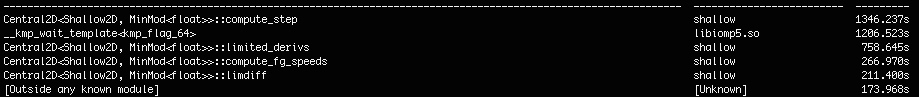
\includegraphics[width=0.7\columnwidth]{collapse_omp}
				\caption{Timing of entire simulation using implementation of OpenMP parallelized for-loops with \texttt{collapse} option. Generated using Intel's VTUNE on Totient.}
				\label{collapse_omp}
			\end{center}
		\end{figure}
\FloatBarrier
	\bibliography{report.bib}
	\bibliographystyle{unsrt}
	
\end{document}